\documentclass{article}
\usepackage[utf8]{inputenc}
\usepackage{multicol}
\usepackage{listings}
\usepackage{amssymb}
\usepackage{enumitem}
\usepackage{graphicx}
\usepackage{amsthm}
\usepackage{hyperref}
\usepackage{tikz}
\usepackage[ruled,vlined]{algorithm2e}
\newtheorem{theorem}{Theorem}
\newtheorem{definition}{Definition}

\usetikzlibrary{arrows, positioning}

\SetKwProg{Fn}{Function}{}{}
\SetKwProg{Proc}{Procedure}{}{}
\SetKwFunction{clientConnect}{clientConnect}
\SetKwFunction{getStationsInRange}{getStationsInRange}
\SetKwFunction{getConnectedClients}{getConnectedClients}

\SetKwFunction{findAdvertisement}{findAdvertisement}
\SetKwFunction{findAdvertisement}{findAdvertisement}
\SetKwFunction{findAdvertisementByDemographicGroup}{findAdvertisementByUsersDemographicGroups}
\SetKwFunction{fordFulkersonMaxFlow}{fordFulkerson}
\SetKwFunction{augment}{augment}
\SetKwFunction{createGraph}{createNetwork}
\SetKwFunction{checkClientConnections}{checkAllClientsCanConnect}
\SetKwFunction{showRandomSuitableAd}{showRandomSuitableAd}

%=====================================
%			Assignment 6
%=====================================

\begin{document}

\title{Weekly Assignment 6}
\date{12th October 2017}
\author{Tony Lopar s1013792}
\maketitle

\paragraph{Deadline:} 18th October 2017, 6pm.
\paragraph{Solutions:} Solutions can be found below the exercises
\paragraph{Collaboration} Some graphs in this document are made in collaboration with Carlo Jessurun. We collaborated with creating the graphs in LaTeX. However, we applied our own solutions in the graphs and descriptions.

\section*{Exercise 1. \textit{Weight: 25\%}}
We want to choose scientific experiments among $n$ experiments $E_1, \ldots E_n$ that must be done in outer space. Each experiment needs tools that should be chosen among $p$ tools $I_1, . . . , I_p$. Each tool may be used by multiple experiments. By conducting the experiment $E_i$, we earn $p_i$ euros, but carrying the tool $I_j$ into outer space costs $c_j$ euros.

The goal is to maximize the profits.

Let us consider the following graph: for each experiment $E_i$, we add a vertex $E_i$. For each tool $I_j$, we add a vertex $I_j$. There is also a source $s$ and a sink $t$. An edge of capacity $p_i$ goes from $s$ to $E_i$ and an edge of capacity $c_j$ goes from $I_j$ to $t$. Finally, if the experiment $E_i$ uses the tool $I_j$ , then there is an edge of infinite capacity from $E_i$ to $I_j$.

\begin{enumerate}
  \item What is the graph associated to the following experiments?

%  	\begin{figure}[h!]
%       \centering
%       \includegraphics[width=6cm]{img/flow-6.PNG}
% 	\end{figure}

  \item How can we find the solution (that is to say, the set of experiments) that maximizes the profits? How can we compute the total profits?
\end{enumerate}

\subsection*{Solutions exercise 1}
\begin{enumerate}
  \item The graph can be found in figure~\ref{fig:M1}
  \item We could do a max flow on the graph and see which projects have a flow from the source that's lower than the max flow while the flow from the instruments used for the experiment to the sink is equal to the capacity. When the flow to the experiment is lower than it's capacity, this means the profits will be higher than the total cost of the project. So, when we execute a max flow on this graph and pick all the experiments that have a flow that's lower than the capacity, then we have found the experiments that may be profitable. To know sure that these experiments are profitable, we have to shrink the flow to the non-profitable experiments to 0 to make sure these experiments didn't make a non-profitable experiment look profitable having a flow from the experiments.

  In order to find the max benefits we may do a max flow search on the graph. After this we should check whether all instruments have a flow to the sink that's equal to their capacity. If this isn't the case, then the experiment can't afford the instrument. The experiments that depend on these instruments will be cancelled, so we set the capacity of this experiments to 0. After this we will execute a max flow with the new capacities and see whether we will make profit on all the experiments. We can compute the profits by taking the residual graph and take the sum of all outgoing edges from the source.
\end{enumerate}
\begin{figure}[ht]
\begin{center}
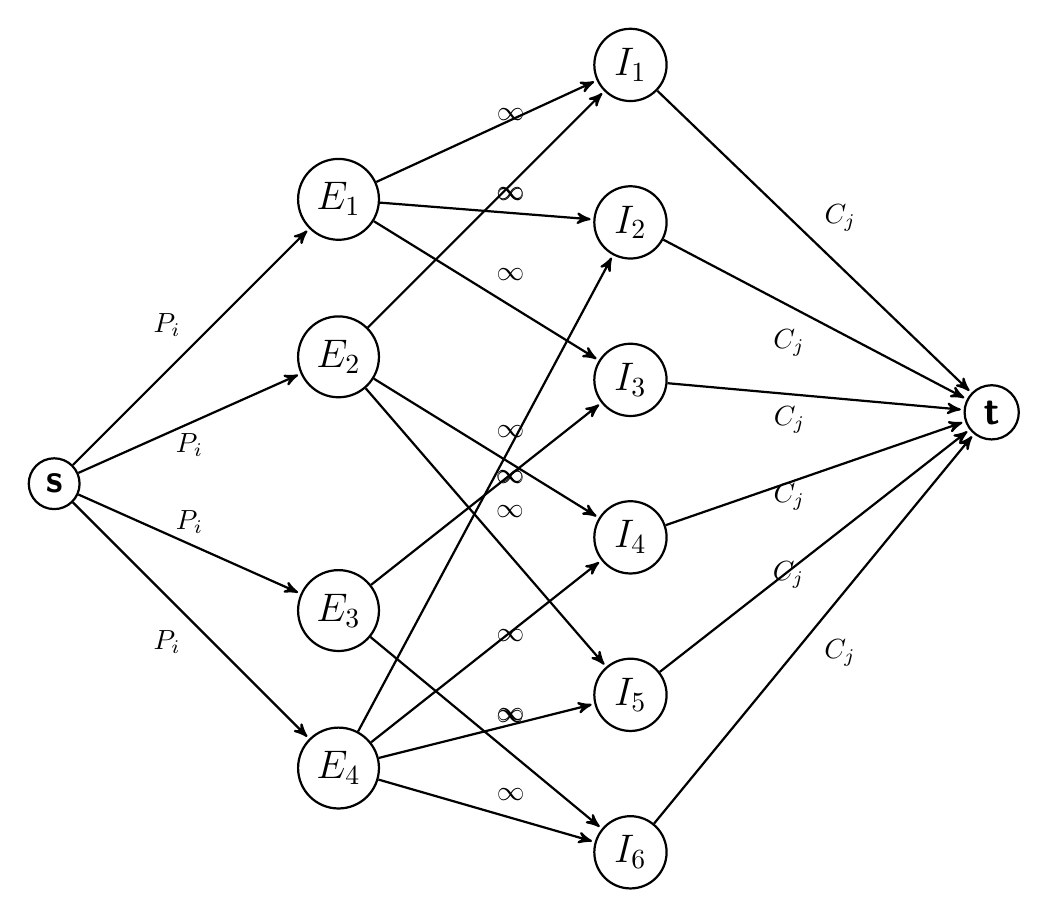
\begin{tikzpicture}[->,>=stealth',shorten >=1pt,auto,node distance=2cm, every loop/.style={},
                    thick, ,main node/.style={circle,draw,font=\sffamily\Large\bfseries}]

  \node[main node] (1) {s};
  \node[main node] (2) [above right=1cm and 3cm of 1] {$E_2$};
  \node[main node] (3) [above of=2] {$E_1$};
  \node[main node] (4) [below right=1cm and 3cm of 1] {$E_3$};
  \node[main node] (5) [below of=4] {$E_4$};
  \node[main node] (6) [above right=1cm and 3cm of 3] {$I_1$};
  \node[main node] (7) [below of=6] {$I_2$};
  \node[main node] (8) [below of=7] {$I_3$};
  \node[main node] (9) [below of=8] {$I_4$};
  \node[main node] (10) [below of=9] {$I_5$};
  \node[main node] (11) [below of=10] {$I_6$};
  \node[main node] (12) [above right=1cm and 4cm of 9] {t};

  \path[every node/.style={font=\sffamily\normalsize, text = black }]
    (1) edge[black] node [below] {$P_i$} (2)
        edge[black] node [above left ] {$P_i$} (3)
        edge[black] node [above] {$P_i$} (4)
        edge[black] node [below left] {$P_i$} (5)
    (2) edge[black] node [above right] {$\infty$} (6)
        edge[black] node [above right] {$\infty$} (9)
        edge[black] node [above right] {$\infty$} (10)
    (3) edge[black] node [above right] {$\infty$} (6)
        edge[black] node [above right] {$\infty$} (7)
        edge[black] node [above right] {$\infty$} (8)
    (4) edge[black] node [above right] {$\infty$} (8)
        edge[black] node [above right] {$\infty$} (11)
    (5) edge[black] node [above right] {$\infty$} (7)
        edge[black] node [above right] {$\infty$} (9)
        edge[black] node [above right] {$\infty$} (10)
        edge[black] node [above right] {$\infty$} (11)
    (6) edge[black] node [above right] {$C_j$} (12)
    (7) edge[black] node [below left] {$C_j$} (12)
    (8) edge[black] node [below left] {$C_j$} (12)
    (9) edge[black] node [below left] {$C_j$} (12)
    (10) edge[black] node [below left] {$C_j$} (12)
    (11) edge[black] node [below right] {$C_j$} (12);
\end{tikzpicture}
\caption{Exeriments graph} \label{fig:M1}
\end{center}
\end{figure}

\newpage
\section*{Exercise 2. \textit{Weight: 25\%}}
Consider a set of mobile computing \emph{clients} in a certain town who each need to be connected to one of several possible \emph{base stations}. There are $n$ clients, with the position of each client specified by its $(x, y)$ coordinates in the plane.
There are also $k$ base stations; the position of each of these is specified by $(x,y)$ coordinates as well.

We wish to connect each client to exactly one of the base stations. Our choice of connection is constrained in the following ways. There is a \emph{range parameter} $r$ --- a client can only be connected to a base station that is within distance $r$. There is also a \emph{load parameter} $L$ --- no more than $L$ clients can be connected to any single station.

Design a polynomial-time algorithm for the following problem. Given the positions of a set of clients and a set of base stations, as well as the range and load parameters, decide whether every client can be connected simultaneously to a base station, subject to the conditions from the previous paragraph.

\subsection*{Solutions exercise 2}
In this algorithm we have try to connect each client to a base station. The condition from a client is that the station is within it's range $R$. A base station has a capacity of $L$ clients that can be connected.

First we should do a bipartite matching between the clients and basestations. In this matching we will only check which basestations are in the range of a client.

When we have the bipartite matching, we can create a network flow by adding a source and a sink. From the source there should go an edge with capacity 1 to all clients and from the basestations an edge with capacity L to the sink. In this network we can run ford-folkerson to find the maximum bipartite matching.

After the execution of ford-folkerson on the network, we may check whether a flow is possible from the source in the residual graph. When there is a flow possible, then we found a client that could not be connected to a basestation. Otherwise we succeeded to connect all clients to a basestation.

In the algorithm I combined the steps of matching and creating a network in the function \createGraph{}. The algorithm has a complexity of $O(|C| \cdot |B|)$, since the matching in the algorithm depends on the number of clients and basestations.

\begin{algorithm}[ht!]
  \DontPrintSemicolon
  \Proc{\checkClientConnections{C, B}}{
    $s \leftarrow vertex$  \;
    $t \leftarrow vertex$ \;
    \fordFulkersonMaxFlow{ \createGraph{s, C, B, t}, s, t} \;
    \If{we can reach a client from the source in the residual graph}{
      \KwRet{false}
    } \Else {
      \KwRet{true}
    }
  }
  \Fn{\createGraph{s, C, B, t}}{
    $vertices \leftarrow nil$ \;
    $edges \leftarrow nil$ \;

    $vertices.add(s)$ \;
    $vertices.add(t)$ \;

      \ForEach{$c \in C$}{
        $vertices.add(c)$ \;
        $s.addEdge(c, 1)$ \;
        \ForEach{$b \in B$} {
          \If{$b \notin vertices$}{
            $vertices.add(b)$ \;
            $b.addEdge(t, L[b])$ \;
          }
          \If{$b.isInRangeOf(c)$}{
            $c.addEdge(b, \infty)$ \;
          }

        }
      }
      \KwRet{$graph \leftarrow \{vertices, edges\}$}
  }

  \Proc{\fordFulkersonMaxFlow{G,s,t}}{
    $G_f \leftarrow residual graph$ \;
       \ForEach{$e \in E : f(e) \leftarrow 0$}{
         \While{there exists an augmenting path P in Gf}{
           $f \leftarrow Augment(f,p)$ \;
           $Update \enspace G_f$ \;
         }
         \KwRet{f}
       }
}
   \Proc{\augment{f,P}}{
     $b \leftarrow  $bottleneck capacity of path P \;
     \ForEach{$e \in P$} {
       \If{$e \in E$} {
         $f(e) \leftarrow f(e) + b$
       } \Else{
         $f(e^R) \leftarrow f(e^R) - b$
       }
     }
   }

  %   \Proc{\clientConnect{}}{
  %     \ForEach{$c \in C$}{
  %       \ForEach{$b \in \getStationsInRange{c}$}{
  %         \If{b.getLoad $>$ \getConnectedClients(b)}{
  %           b.addClient(c) \;
  %           \textbf{continue} \;
  %         }
  %       }
  %     }
  % }
    \caption{Algorithm for connecting clients to base stations}
\end{algorithm}

\newpage
\section*{Exercise 3. \textit{Weight: 25\%}}
Suppose you are organizing a conference where researchers present articles they have written. Researchers who want to present an article send a paper to the conference organizers. The
conference organizers have access to a set $A$ of reviewers who are each willing to read up to $m_A$
articles. Let $B$ the set of papers to review: each gets reviewed by up to $m_B$ reviewers. Moreover, each submission has a particular topic and each reviewer has a specialization for a set of topics, so papers on a given topic only get reviewed by those reviewers who are experts on that topic. The conference organizers need to decide which reviewers will review each article (or equivalently, which articles will be reviewed by which reviewers). Explain how this problem can be solved using a flow network.

\subsection*{Solutions exercise 3}
We can solve this problem by adding the set of all reviewers and papers in a network flow. Before this, we should do a bipartite matching to find out whether the reviewer has a specialization in the topic the paper is about. Since I assume that each reviewer will review a paper only once, the capacity of the flows between the reviewers and papers will be 1. The reviewers will have an flow from the source with capacity $m_A$ and each paper will have an flow to the sink with capacity $m_B$.

In order to get a maximum matching, we could run ford-folkerson on the algorithm. In the resulting residual graph, there will be edges from the papers to the reviewers. So, for every paper we have a flow to the reviewers that will review it.

An example of a network flow with 3 reviewers with specializations in different topics and 4 papers can be found in figure~\ref{fig:M2}. The edges between A and B are found in the bipartite matching of the topic.
\begin{figure}[ht]
\begin{center}
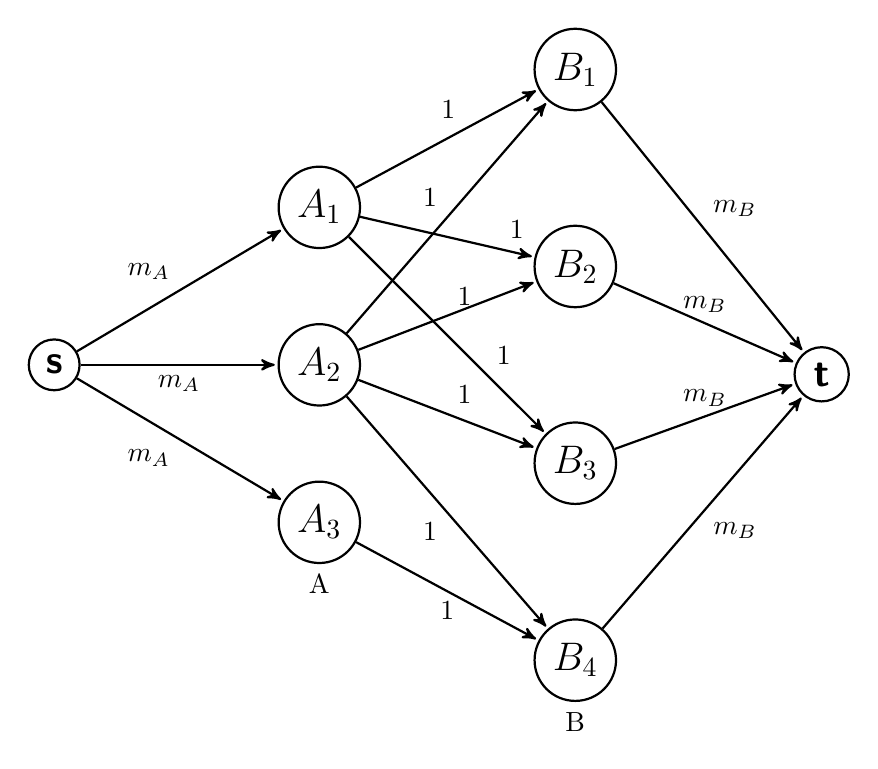
\begin{tikzpicture}[->,>=stealth',shorten >=1pt,auto,node distance=2cm, every loop/.style={},thick, ,main node/.style={circle,draw,font=\sffamily\Large\bfseries}]

  \node[main node] (1) {s};
  \node[main node] (2) [right=1cm and 2.5cm of 1] {$A_2$};
  \node[main node] (3) [above of=2] {$A_1$};
  \node[main node][label = {[align=center]below:A}] (4) [below of=2]{$A_3$};
  % \node[main node] (5) [above right=1cm and 2.5cm of 2] {$T_1$};
  % \node[main node] (6) [below right=1cm and 2.5cm of 2] {$T_2$};
  \node[main node] (7) [above right=1cm and 2.5cm of 3] {$B_1$};
  \node[main node] (8) [below right=0cm and 2.5cm of 3] {$B_2$};
  \node[main node] (9) [above right=0cm and 2.5cm of 4] {$B_3$};
  \node[main node][label = {[align=center]below:B}] (10) [below right=1cm and 2.5cm of 4] {$B_4$};
  \node[main node] (11) [above right=0.5cm and 2.5cm of 9] {t};

  \path[every node/.style={font=\sffamily\normalsize, text = black }]
    (1) edge[black] node [below] {$m_A$} (2)
        edge[black] node [above left] {$m_A$} (3)
        edge[black] node [below left] {$m_A$} (4)
    (2) edge[black] node [above left] {$1$} (7)
        edge[black] node [above right] {$1$} (8)
        edge[black] node [above right] {$1$} (9)
        edge[black] node [below left] {$1$} (10)
    (3) edge[black] node [above left, pos=0.6] {$1$} (7)
        edge[black] node [above right, pos=0.8] {$1$} (8)
        edge[black] node [above right, pos=0.7] {$1$} (9)
    (4) edge[black] node [below] {$1$} (10)
    (7) edge[black] node [above right] {$m_B$} (11)
    (8) edge[black] node [above] {$m_B$} (11)
    (9) edge[black] node [above] {$m_B$} (11)
    (10) edge[black] node [below right] {$m_B$} (11);
\end{tikzpicture}
\caption{Example network flow conference} \label{fig:M2}
\end{center}
\end{figure}

\newpage
\section*{Exercise 4. \textit{Weight: 25\%}}
The managers of a popular website have identified $k$ distinct \emph{demographic groups} $G_1, G_2 ,\ldots, G_k$.
These groups may overlap; for example $G_1$ can be equal to all residents of Gelderland, and $G_2$ can be equal
to all people with a degree in computer science.
The site has contracts with $m$ different \emph{advertisers}, to show a certain number of copies of their ads to users
of the site. Here's what the contract with the $i^{th}$ advertiser looks like:
\begin{itemize}
\item
For a subset $X_i \subseteq \{ G_1 ,\ldots, G_n \}$ of the demographic groups, advertiser $i$ wants its ads shown only to
users who belong to at least one of the groups in the set $X_i$.
\item
Advertiser $i$ wants its ads shown to at least $r_i$ users each minute, for some number $r_i$.
\end{itemize}

Now consider the problem of designing a good \emph{advertising policy} --- a way to show a single ad to each user of the site.
Suppose at a given minute, there are $n$ users visiting the site.
Because we have registration information on each of these users, we know that user $j$ belongs to a subset
$U_j \subseteq \{ G_1 ,\ldots, G_k \}$ of the demographic groups.
Is there a way to show a single ad to each user so that the site's contracts with each of the $m$ advertisers is satisfied
for this minute?

Give an efficient algorithm to decide if this is possible, and if so, to actually choose an ad to show to each user.

\subsection*{Solutions exercise 4}
We may solve this problem using a network flow. For this algorithm we first have to perform a matching between users and advertisers. There is a match when the user and advertiser have a common demographic group. So when we have an intersection between these two sets, then the advertisement can be shown to the user.

After this matching we can add a source and sink to make a network of the problem. There should go an edge from the source to all advertisers with capacity $r_i$. From the users there will be an edge with capacity 1 to the sink.

If we run ford-folkerson we can connect a advertisement of each advertiser to multiple users. When we take the residual graph and we may flow from the source to an advertiser, then we failed to satisfy the minimum views for this advertiser in that minute.

The only remaining problem is when there are more users than the sum or $r_i$ foreach advertiser, because some flows to the advertisers are at their capacity. So, after running Ford-folkerson we will iterate through all users and check whether we already shown a advertisement to them. If this is not the case, we will pick a random advertisement with a common demographic group as the user.

% For this algorithm we should first decide the percentage of demographic groups in the users and advertisements. If we have many advertisements that can only be shown to a small amount of users, we have to give this advertisement priority relative to an advertisement we may show to a demographic group with a lot of users.
% Furthermore, we should count the number of views of the advertisement. If this is lower than $r_i$, then we should try to make it greater or equal.
%
% In the algorithm we should first check which advertisements the user could see. These are the advertisements with at least one demographic group $g \in X_i$ and $g \in U_j$. Now we know all the possible advertisements, we should check whether there are advertisements with less views than $r_i$. If this is the case, we should prefer one of these advertisements to show. To improve the chance that all advertisements are seen more or equal times than $r_i$ we could prioritize in this last step the advertisements with the least possible users to view it.

% \begin{algorithm}[ht!]
%   \DontPrintSemicolon
%
%     \Proc{\findAdvertisement{}}{
%     $possibleAdvertisements \leftarrow nil$ \;
%       \ForEach{$a \in$ \findAdvertisementByDemographicGroup{$U_j$}}{
%         \If{$views[a] < r_i[a]$}{
%             \KwRet{a} \;
%         } \Else{
%           $possibleAdvertisements.add(a)$ \;
%         }
%         $random \leftarrow$ a random integer $\leq$ the number of possible ads \;
%         \KwRet{$possibleAdvertisements[random]$}
%       }
%
%       \KwRet{"No suitable advertisement found"}
%     }
%
%     \Proc{\findAdvertisementByDemographicGroup{$U_j$}}{
%     $possibleAdvertisements \leftarrow nil$ \;
%       \ForEach{$a \in advertisememts$}{
%         \If{$g \in U_j \& g \in X_a$}{
%           $possibleAvertisements.add[a]$
%         }
%       }
%       \KwRet{$advertisements[U_j \cup X_i]$}
%     }
%     \caption{Advertisement policy algorithm}
% \end{algorithm}

\begin{algorithm}[ht!]
  \DontPrintSemicolon
  \Proc{\findAdvertisement{U, M}}{
    $s \leftarrow vertex$  \;
    $t \leftarrow vertex$ \;
    \fordFulkersonMaxFlow{ \createGraph{s, U, M, t}, s, t} \;
    \ForEach{$u \in U$}{
      \If{$f(u) = 0$}{
        \showRandomSuitableAd{} \;
      }
    }
    \If{we can reach an advertiser from the source in the residual graph}{
      \KwRet{false}
    } \Else {
      \KwRet{true}
    }
  }
  \Fn{\createGraph{s, U, M, t}}{
    $vertices \leftarrow nil$ \;
    $edges \leftarrow nil$ \;

    $vertices.add(s)$ \;
    $vertices.add(t)$ \;

      \ForEach{$m \in M$}{
        $vertices.add(m)$ \;
        $s.addEdge(m, r_i)$ \;
        \ForEach{$u \in U$} {
          \If{$u \notin vertices$}{
            $vertices.add(u)$ \;
            $b.addEdge(t, 1)$ \;
          }
          \If{b $\&$ u have a common demographic group}{
            $c.addEdge(b, \infty)$ \;
          }

        }
      }
      \KwRet{$graph \leftarrow \{vertices, edges\}$}
  }

  \Proc{\fordFulkersonMaxFlow{G,s,t}}{
    $G_f \leftarrow residual graph$ \;
       \ForEach{$e \in E : f(e) \leftarrow 0$}{
         \While{there exists an augmenting path P in Gf}{
           $f \leftarrow Augment(f,p)$ \;
           $Update \enspace G_f$ \;
         }
         \KwRet{f}
       }
}
   \Proc{\augment{f,c,P}}{
     $b \leftarrow  $bottleneck capacity of path P \;
     \ForEach{$e \in P$} {
       \If{$e \in E$} {
         $f(e) \leftarrow f(e) + b$
       } \Else{
         $f(e^R) \leftarrow f(e^R) - b$
       }
     }
   }
    \caption{Advertisement policy algorithm}
\end{algorithm}

\end{document}
